%%%%%%%%%%%%%%%%%%%%%%%%%%%%%%%%%%%%%%%%%%%%%%%%%%%%%%%%%%%

%%%%%%%%%%%%%%%%%%%%%%%%%%%%%%%%%%%%%%%%%%%%%%%%%%%%%%%%%%%

%% document class
\documentclass[a4paper,11pt,oneside]{book}

%% packages
%% packages

\usepackage{blindtext} % needed for creating dummy text passages
%\usepackage{ngerman} % needed for German default language
\usepackage{amsmath} % needed for command eqref
\usepackage{amssymb} % needed for math fonts
\usepackage[
	colorlinks=true
	,breaklinks
	%,ngerman
	]{hyperref} % needed for creating hyperlinks in the document, the option colorlinks=true gets rid of the awful boxes, breaklinks breaks lonkg links (list of figures), and ngerman sets everything for german as default hyperlinks language
\usepackage[hyphenbreaks]{breakurl} % ben�tigt f�r das Brechen von URLs in Literaturreferenzen, hyphenbreaks auch bei links, die �ber eine Seite gehen (mit hyphenation).
\usepackage{xcolor}
\definecolor{c1}{rgb}{0,0,1} % blue
\definecolor{c2}{rgb}{0,0.3,0.9} % light blue
\definecolor{c3}{rgb}{0.3,0,0.9} % red blue
\hypersetup{
    linkcolor={c1}, % internal links
    citecolor={c2}, % citations
    urlcolor={c3} % external links/urls
}
%\usepackage{cite} % needed for cite
\usepackage[round,authoryear]{natbib} % needed for cite and abbrvnat bibliography style
\usepackage[nottoc]{tocbibind} % needed for displaying bibliography and other in the table of contents
\usepackage{graphicx} % needed for \includegraphics 
\usepackage{longtable} % needed for long tables over pages
\usepackage{bigstrut} % needed for the command \bigstrut
\usepackage{enumerate} % needed for some options in enumerate
\usepackage{array}
\usepackage{textgreek}
\usepackage{todonotes} % needed for todos
\usepackage{makeidx} % needed for creating an index
\makeindex
\usepackage{placeins}
\usepackage [english]{babel}
\usepackage [autostyle, english = american]{csquotes}
\MakeOuterQuote{"}
\usepackage{multirow}
\usepackage{dcolumn}
\usepackage{array}
\usepackage{makecell}

%% page settings
%% page settings

\usepackage[top=2cm, bottom=1.8cm,left=2.5cm,right=2.5cm]{geometry} % needed for page border settings
\parindent=0cm % for space of first line of new text block
\sloppy % for writing with hyphenless justification (tries to)
\hyphenation{} % use hyphenation of tolerance parameters, http://www.jr-x.de/publikationen/latex/tipps/zeilenumbruch.html
\hyphenpenalty=10000
\exhyphenpenalty=10000
\usepackage{fancyhdr} % needed for head and foot options

%% own commands
%\newcommand{\tbi}[1]{\textbf{\textit{#1}}}
%% my macros

%% Text fomats
\newcommand{\tbi}[1]{\textbf{\textit{#1}}}

%% Math fonts
\newcommand{\bbA}{\mathbb{A}}
\newcommand{\bbB}{\mathbb{B}}
\newcommand{\bbC}{\mathbb{C}}
\newcommand{\bbD}{\mathbb{D}}
\newcommand{\bbE}{\mathbb{E}}
\newcommand{\bbF}{\mathbb{F}}
\newcommand{\bbG}{\mathbb{G}}
\newcommand{\bbH}{\mathbb{H}}
\newcommand{\bbI}{\mathbb{I}}
\newcommand{\bbJ}{\mathbb{J}}
\newcommand{\bbK}{\mathbb{K}}
\newcommand{\bbL}{\mathbb{L}}
\newcommand{\bbM}{\mathbb{M}}
\newcommand{\bbN}{\mathbb{N}}
\newcommand{\bbO}{\mathbb{O}}
\newcommand{\bbP}{\mathbb{P}}
\newcommand{\bbQ}{\mathbb{Q}}
\newcommand{\bbR}{\mathbb{R}}
\newcommand{\bbS}{\mathbb{S}}
\newcommand{\bbT}{\mathbb{T}}
\newcommand{\bbU}{\mathbb{U}}
\newcommand{\bbV}{\mathbb{V}}
\newcommand{\bbW}{\mathbb{W}}
\newcommand{\bbX}{\mathbb{X}}
\newcommand{\bbY}{\mathbb{Y}}
\newcommand{\bbZ}{\mathbb{Z}}
\newcommand{\imp}[1]{\underline{\textit{#1}}}

%%%%%%%%%%%%%%%%%%%%%%%%%%%%%%%%%%%%%%%%%%%%%%%%%%%%%%%%%%%

\begin{document}
	
	%%%%%%%%%%%%%%%%%%%%%%%%%%%%%%%%%%%%%%%%%%%%%%%%%%%%%%%%%%%
	%%%%%%%%%%%%%%%%%%%%%%%%%%%%%%%%%%%%%%%%%%%%%%%%%%%%%%%%%%%
	%%%%%%%%%%%%%%%%%%%%%%%%%%%%%%%%%%%%%%%%%%%%%%%%%%%%%%%%%%%
	
	%\pagestyle{empty}
	%\title{Basic elements for writing a book/thesis using \LaTeX}
	%\author{Mauricio Lobos}
	%\date{}
	%\maketitle
	%%%%%%%%%%%%%%%%%%%%%%%%%%%%%%%%%%%%%%%%%
% University Assignment Title Page 
% LaTeX Template
% Version 1.0 (27/12/12)
%
% This template has been downloaded from:
% http://www.LaTeXTemplates.com
%
% Original author:
% WikiBooks (http://en.wikibooks.org/wiki/LaTeX/Title_Creation)
%
% License:
% CC BY-NC-SA 3.0 (http://creativecommons.org/licenses/by-nc-sa/3.0/)
% 
% Instructions for using this template:
% This title page is capable of being compiled as is. This is not useful for 
% including it in another document. To do this, you have two options: 
%
% 1) Copy/paste everything between \begin{document} and \end{document} 
% starting at \begin{} and paste this into another LaTeX file where you 
% want your title page.
% OR
% 2) Remove everything outside the \begin{titlepage} and \end{titlepage} and 
% move this file to the same directory as the LaTeX file you wish to add it to. 
% Then add %%%%%%%%%%%%%%%%%%%%%%%%%%%%%%%%%%%%%%%%%
% University Assignment Title Page 
% LaTeX Template
% Version 1.0 (27/12/12)
%
% This template has been downloaded from:
% http://www.LaTeXTemplates.com
%
% Original author:
% WikiBooks (http://en.wikibooks.org/wiki/LaTeX/Title_Creation)
%
% License:
% CC BY-NC-SA 3.0 (http://creativecommons.org/licenses/by-nc-sa/3.0/)
% 
% Instructions for using this template:
% This title page is capable of being compiled as is. This is not useful for 
% including it in another document. To do this, you have two options: 
%
% 1) Copy/paste everything between \begin{document} and \end{document} 
% starting at \begin{} and paste this into another LaTeX file where you 
% want your title page.
% OR
% 2) Remove everything outside the \begin{titlepage} and \end{titlepage} and 
% move this file to the same directory as the LaTeX file you wish to add it to. 
% Then add %%%%%%%%%%%%%%%%%%%%%%%%%%%%%%%%%%%%%%%%%
% University Assignment Title Page 
% LaTeX Template
% Version 1.0 (27/12/12)
%
% This template has been downloaded from:
% http://www.LaTeXTemplates.com
%
% Original author:
% WikiBooks (http://en.wikibooks.org/wiki/LaTeX/Title_Creation)
%
% License:
% CC BY-NC-SA 3.0 (http://creativecommons.org/licenses/by-nc-sa/3.0/)
% 
% Instructions for using this template:
% This title page is capable of being compiled as is. This is not useful for 
% including it in another document. To do this, you have two options: 
%
% 1) Copy/paste everything between \begin{document} and \end{document} 
% starting at \begin{} and paste this into another LaTeX file where you 
% want your title page.
% OR
% 2) Remove everything outside the \begin{titlepage} and \end{titlepage} and 
% move this file to the same directory as the LaTeX file you wish to add it to. 
% Then add \input{./title_page_1.tex} to your LaTeX file where you want your
% title page.
%
%%%%%%%%%%%%%%%%%%%%%%%%%%%%%%%%%%%%%%%%%

%----------------------------------------------------------------------------------------
%	PACKAGES AND OTHER DOCUMENT CONFIGURATIONS
%----------------------------------------------------------------------------------------

%\documentclass[12pt]{article}
%
%\begin{document}

\begin{titlepage}
	

\newcommand{\HRule}{\rule{\linewidth}{0.5mm}} % Defines a new command for the horizontal lines, change thickness here

\center % Center everything on the page
 
%----------------------------------------------------------------------------------------
%	HEADING SECTIONS
%----------------------------------------------------------------------------------------
\begin{minipage}[b]{0.4\textwidth}
	%\begin{flushleft} \large
	\begin{center}
		
\includegraphics[width=0.5\textwidth]{figures/download}\\[1cm] % Include a department/university logo - this will require the graphicx package
		%\end{flushleft}
	\end{center}
\end{minipage}
\vspace{1.5cm}



\textsc{\LARGE Department of Financial Mathematics}\\[1.5cm] % Name of your university/college
\textsc{\Large }\\[0.5cm] % Major heading such as course name
\textsc{\large }\\[0.5cm] % Minor heading such as course title

%----------------------------------------------------------------------------------------
%	TITLE SECTION
%----------------------------------------------------------------------------------------

\HRule \\[0.5cm]
{ \huge \bfseries Comparison of Forecasting Models for Value at Risk}\\[0.1cm] % Title of your document
\HRule \\[1.5cm]
\vspace{2.5cm}
 
%----------------------------------------------------------------------------------------
%	AUTHOR SECTION
%----------------------------------------------------------------------------------------


\begin{minipage}{0.4\textwidth}
\begin{flushleft} \large
\emph{Author:}\\
Hafees Adebayo \textsc{Yusuff} % Your name
\end{flushleft}
\end{minipage}
~
\begin{minipage}{0.4\textwidth}
\begin{flushleft} \large
\emph{Supervisor:} \\
Prof. Ralf \textsc{Korn} % Supervisor's Name
\end{flushleft}
\end{minipage}\\[4cm]

% If you don't want a supervisor, uncomment the two lines below and remove the section above
%\Large \emph{Author:}\\
%John \textsc{Smith}\\[3cm] % Your name

%----------------------------------------------------------------------------------------

%	DATE SECTION
%----------------------------------------------------------------------------------------

{\large \today}\\[3cm] % Date, change the \today to a set date if you want to be precise
\vspace{2.5cm}


A thesis submitted in fulfilment of the requirements for the degree of
Master of Science

%----------------------------------------------------------------------------------------
%	LOGO SECTION
%----------------------------------------------------------------------------------------

%~
%\begin{minipage}[b]{0.4\textwidth}
%\begin{flushleft} \large
%
\includegraphics[width=0.5\textwidth]{figures/download (1)}
%\end{flushleft}
%\end{minipage}

%----------------------------------------------------------------------------------------

\vfill % Fill the rest of the page with whitespace
\end{titlepage}



\thispagestyle{empty}

\newpage\null\thispagestyle{empty}\newpage


\begin{titlepage}
	\textbf{\LARGE Declaration of Authorship}\newline\newline
	

		
		I, Hafees Adebayo YUSUFF, hereby declare the following thesis titled "Comparison of forecasting models for value at risk" to be my own work and I confirm that:
			\begin{itemize}
		\item[$\bullet$] The thesis I am submitting is entirely my own work except where otherwise indicated.
		
		\item[$\bullet$] It has not been submitted, either partially or in full, for a qualification at this or any other University.
	
	\item[$\bullet$] I have clearly signalled the presence of all material I have quoted from other sources,
	including any diagrams, charts, tables or graphs.
	
	\item[$\bullet$] I have acknowledged appropriately any assistance I have received.
	
	\end{itemize}
	
	\vspace*{4em}\noindent
	\hfill%
	\begin{tabular}[t]{c}
		\rule{10em}{0.4pt}\\ Signature
	\end{tabular}%
	\hfill%
	\begin{tabular}[t]{c}
		\rule{10em}{0.4pt}\\ Date
	\end{tabular}%
	\hfill\strut


\end{titlepage}
 to your LaTeX file where you want your
% title page.
%
%%%%%%%%%%%%%%%%%%%%%%%%%%%%%%%%%%%%%%%%%

%----------------------------------------------------------------------------------------
%	PACKAGES AND OTHER DOCUMENT CONFIGURATIONS
%----------------------------------------------------------------------------------------

%\documentclass[12pt]{article}
%
%\begin{document}

\begin{titlepage}
	

\newcommand{\HRule}{\rule{\linewidth}{0.5mm}} % Defines a new command for the horizontal lines, change thickness here

\center % Center everything on the page
 
%----------------------------------------------------------------------------------------
%	HEADING SECTIONS
%----------------------------------------------------------------------------------------
\begin{minipage}[b]{0.4\textwidth}
	%\begin{flushleft} \large
	\begin{center}
		
\includegraphics[width=0.5\textwidth]{figures/download}\\[1cm] % Include a department/university logo - this will require the graphicx package
		%\end{flushleft}
	\end{center}
\end{minipage}
\vspace{1.5cm}



\textsc{\LARGE Department of Financial Mathematics}\\[1.5cm] % Name of your university/college
\textsc{\Large }\\[0.5cm] % Major heading such as course name
\textsc{\large }\\[0.5cm] % Minor heading such as course title

%----------------------------------------------------------------------------------------
%	TITLE SECTION
%----------------------------------------------------------------------------------------

\HRule \\[0.5cm]
{ \huge \bfseries Comparison of Forecasting Models for Value at Risk}\\[0.1cm] % Title of your document
\HRule \\[1.5cm]
\vspace{2.5cm}
 
%----------------------------------------------------------------------------------------
%	AUTHOR SECTION
%----------------------------------------------------------------------------------------


\begin{minipage}{0.4\textwidth}
\begin{flushleft} \large
\emph{Author:}\\
Hafees Adebayo \textsc{Yusuff} % Your name
\end{flushleft}
\end{minipage}
~
\begin{minipage}{0.4\textwidth}
\begin{flushleft} \large
\emph{Supervisor:} \\
Prof. Ralf \textsc{Korn} % Supervisor's Name
\end{flushleft}
\end{minipage}\\[4cm]

% If you don't want a supervisor, uncomment the two lines below and remove the section above
%\Large \emph{Author:}\\
%John \textsc{Smith}\\[3cm] % Your name

%----------------------------------------------------------------------------------------

%	DATE SECTION
%----------------------------------------------------------------------------------------

{\large \today}\\[3cm] % Date, change the \today to a set date if you want to be precise
\vspace{2.5cm}


A thesis submitted in fulfilment of the requirements for the degree of
Master of Science

%----------------------------------------------------------------------------------------
%	LOGO SECTION
%----------------------------------------------------------------------------------------

%~
%\begin{minipage}[b]{0.4\textwidth}
%\begin{flushleft} \large
%
\includegraphics[width=0.5\textwidth]{figures/download (1)}
%\end{flushleft}
%\end{minipage}

%----------------------------------------------------------------------------------------

\vfill % Fill the rest of the page with whitespace
\end{titlepage}



\thispagestyle{empty}

\newpage\null\thispagestyle{empty}\newpage


\begin{titlepage}
	\textbf{\LARGE Declaration of Authorship}\newline\newline
	

		
		I, Hafees Adebayo YUSUFF, hereby declare the following thesis titled "Comparison of forecasting models for value at risk" to be my own work and I confirm that:
			\begin{itemize}
		\item[$\bullet$] The thesis I am submitting is entirely my own work except where otherwise indicated.
		
		\item[$\bullet$] It has not been submitted, either partially or in full, for a qualification at this or any other University.
	
	\item[$\bullet$] I have clearly signalled the presence of all material I have quoted from other sources,
	including any diagrams, charts, tables or graphs.
	
	\item[$\bullet$] I have acknowledged appropriately any assistance I have received.
	
	\end{itemize}
	
	\vspace*{4em}\noindent
	\hfill%
	\begin{tabular}[t]{c}
		\rule{10em}{0.4pt}\\ Signature
	\end{tabular}%
	\hfill%
	\begin{tabular}[t]{c}
		\rule{10em}{0.4pt}\\ Date
	\end{tabular}%
	\hfill\strut


\end{titlepage}
 to your LaTeX file where you want your
% title page.
%
%%%%%%%%%%%%%%%%%%%%%%%%%%%%%%%%%%%%%%%%%

%----------------------------------------------------------------------------------------
%	PACKAGES AND OTHER DOCUMENT CONFIGURATIONS
%----------------------------------------------------------------------------------------

%\documentclass[12pt]{article}
%
%\begin{document}

\begin{titlepage}
	

\newcommand{\HRule}{\rule{\linewidth}{0.5mm}} % Defines a new command for the horizontal lines, change thickness here

\center % Center everything on the page
 
%----------------------------------------------------------------------------------------
%	HEADING SECTIONS
%----------------------------------------------------------------------------------------
\begin{minipage}[b]{0.4\textwidth}
	%\begin{flushleft} \large
	\begin{center}
		
\includegraphics[width=0.5\textwidth]{figures/download}\\[1cm] % Include a department/university logo - this will require the graphicx package
		%\end{flushleft}
	\end{center}
\end{minipage}
\vspace{1.5cm}



\textsc{\LARGE Department of Financial Mathematics}\\[1.5cm] % Name of your university/college
\textsc{\Large }\\[0.5cm] % Major heading such as course name
\textsc{\large }\\[0.5cm] % Minor heading such as course title

%----------------------------------------------------------------------------------------
%	TITLE SECTION
%----------------------------------------------------------------------------------------

\HRule \\[0.5cm]
{ \huge \bfseries Comparison of Forecasting Models for Value at Risk}\\[0.1cm] % Title of your document
\HRule \\[1.5cm]
\vspace{2.5cm}
 
%----------------------------------------------------------------------------------------
%	AUTHOR SECTION
%----------------------------------------------------------------------------------------


\begin{minipage}{0.4\textwidth}
\begin{flushleft} \large
\emph{Author:}\\
Hafees Adebayo \textsc{Yusuff} % Your name
\end{flushleft}
\end{minipage}
~
\begin{minipage}{0.4\textwidth}
\begin{flushleft} \large
\emph{Supervisor:} \\
Prof. Ralf \textsc{Korn} % Supervisor's Name
\end{flushleft}
\end{minipage}\\[4cm]

% If you don't want a supervisor, uncomment the two lines below and remove the section above
%\Large \emph{Author:}\\
%John \textsc{Smith}\\[3cm] % Your name

%----------------------------------------------------------------------------------------

%	DATE SECTION
%----------------------------------------------------------------------------------------

{\large \today}\\[3cm] % Date, change the \today to a set date if you want to be precise
\vspace{2.5cm}


A thesis submitted in fulfilment of the requirements for the degree of
Master of Science

%----------------------------------------------------------------------------------------
%	LOGO SECTION
%----------------------------------------------------------------------------------------

%~
%\begin{minipage}[b]{0.4\textwidth}
%\begin{flushleft} \large
%
\includegraphics[width=0.5\textwidth]{figures/download (1)}
%\end{flushleft}
%\end{minipage}

%----------------------------------------------------------------------------------------

\vfill % Fill the rest of the page with whitespace
\end{titlepage}



\thispagestyle{empty}

\newpage\null\thispagestyle{empty}\newpage


\begin{titlepage}
	\textbf{\LARGE Declaration of Authorship}\newline\newline
	

		
		I, Hafees Adebayo YUSUFF, hereby declare the following thesis titled "Comparison of forecasting models for value at risk" to be my own work and I confirm that:
			\begin{itemize}
		\item[$\bullet$] The thesis I am submitting is entirely my own work except where otherwise indicated.
		
		\item[$\bullet$] It has not been submitted, either partially or in full, for a qualification at this or any other University.
	
	\item[$\bullet$] I have clearly signalled the presence of all material I have quoted from other sources,
	including any diagrams, charts, tables or graphs.
	
	\item[$\bullet$] I have acknowledged appropriately any assistance I have received.
	
	\end{itemize}
	
	\vspace*{4em}\noindent
	\hfill%
	\begin{tabular}[t]{c}
		\rule{10em}{0.4pt}\\ Signature
	\end{tabular}%
	\hfill%
	\begin{tabular}[t]{c}
		\rule{10em}{0.4pt}\\ Date
	\end{tabular}%
	\hfill\strut


\end{titlepage}
 % downloaded template
	
	%\pagestyle{plain}
	%\listoftodos
	\tableofcontents
	
	%%%%%%%%%%%%%%%%%%%%%%%%%%%%%%%%%%%%%%%%%%%%%%%%%%%%%%%%%%%
	%%%%%%%%%%%%%%%%%%%%%%%%%%%%%%%%%%%%%%%%%%%%%%%%%%%%%%%%%%%
	%%%%%%%%%%%%%%%%%%%%%%%%%%%%%%%%%%%%%%%%%%%%%%%%%%%%%%%%%%%


%%%%%%%%%%%%%%%%%%%%%%%%%%%%%%%%%%%%%%%%%%%%%%%%%%%%%%%%%%%
%%%%%%%%%%%%%%%%%%%%%%%%%%%%%%%%%%%%%%%%%%%%%%%%%%%%%%%%%%%
%%%%%%%%%%%%%%%%%%%%%%%%%%%%%%%%%%%%%%%%%%%%%%%%%%%%%%%%%%%

\chapter{Introduction}



%%%%%%%%%%%%%%%%%%%%%%%%%%%%%%%%%%%%%%%%%%%%%%%%%%%%%%%%%%%
%%%%%%%%%%%%%%%%%%%%%%%%%%%%%%%%%%%%%%%%%%%%%%%%%%%%%%%%%%%

\section{Motivation}

Basel I (Basel Accord) is the agreement reached
in 1988 in Basel (Switzerland) by the Basel Committee on Bank
Supervision (BCBS), involving the chairmen of the central banks
of some European countries and
the United States of America. This accord provides recommendations
on banking regulations with regard to credit, market and
operational risks. It aims to ensure that financial institutions
hold enough capital on account to meet obligations and absorb
unexpected losses. \newline\newline
For a financial institution measuring the risk it faces is an essential
task. In the specific case of market risk, a possible method of
measurement is the evaluation of losses likely to be incurred when
the price of the portfolio assets falls. This is what Value at Risk
(VaR) does.\newline\newline
Value at Risk(VaR) is the most common way of measuring market risk. It determines the greatest possible loss, assuming an $\alpha$ significance level under a normal market condition at a set time period.\newline\newline
Many VaR estimation methods have been developed in order to reduced uncertainty. It is however of interest to compare these method and determine the prevalence of one VaR estimation approach over others.






%%%%%%%%%%%%%%%%%%%%%%%%%%%%%%%%%%%%%%%%%%%%%%%%%%%%%%%%%%%



\section{Literature review}

The first papers involving the comparison of VaR methodologies, such as those by Beder (1995, 1996), Hendricks (1996), and
Pritsker (1997), reported that the Historical Simulation performed at least as well as the methodologies developed in the early years, the Parametric approach and the Monte Carlo simulation. These papers conclude that among earlier methods, no approach appeared to perform better than the
others. The evaluation and categorization of models carried out in the work by McAleer, Jimenez-Martin and Perez-Amaral(2009) and Shams and Sina (2014), among others, try to determine the conditions under which certain models predict the best. Researchers compared models in periods of varying volatility-before the crisis and after the crisis (When there was no high volatility and when volatility was high, respectively). However, this confirms that some models have good predictions before the start of the crisis, but their quality reduces with increased volatility. Others are more conservative during periods of low volatility, but in the time of the crisis the number of errors made by these models is relatively low.
\newline\newline
Bao et al.(2006), Consigli(2002) and Danielson(2002), among
others, show that in stable periods, parametric models provide satisfactory results
that become less satisfactory during high volatility periods.  Additional studies that find
evidence in favour of parametric methods are Sarma et al.(2003), who compare
Historical simulation and Parametric methods, and Danielson and Vries(2000) in a
similar comparison that also includes Extreme value theory methods. Chong(2004),
who uses parametric methods to estimate VaR under a Normal distribution and under a
Student’s t-distribution, finds a better performance under Normality. McAleer et al.(2009) showed that RiskMetrics\textsuperscript{TM} was
the best fitted model during a crisis, while Shams and Sina(2014) recognized GARCH(1,1) and GJR-GARCH as well
forecasting models. In contrast to the results obtained
by McAleer et al.(2009), the level of quality of forecasts
generated by the RiskMetrics\textsuperscript{TM} model was considered
unsatisfactory by them. However, attention needs to be
drawn to one difference in the samples, on which the
study was conducted, i.e. the first one comes from a
developed country (USA, S\&P500), and the second one
from a developing country (Iran, TSEM). Taylor(2020) evaluate Value at Risk using quantile skill score and the conditional autoregressive model outperformed others.
\newline\newline

Attempts have been made to predicts VaR with ANN. VaR estimation on the exchange rate market in the context of ANNs is dealt with in
Locarek-Junge and Prinzler (1999), who illustrate how VaR estimates can be obtained
by using a USD-portfolio. The empirical outcomes demonstrate an evident superiority
of the neural network to other VaR models. Hamid and Iqbal(2004) compared volatility forecasts from neural networks with forecasts of implied volatility from S\&P500 index futures options, using the Barone-Adesi and Whaley (BAW) American futures options pricing model. Forecasts from NN outperformed implied volatility forecasts. Similar results are put forth by He et al.
(2018), who propose an innovative EMD-DBN type of ANN to estimate VaR on the
USD against the AUD, CAD, CHF and the EUR. The authors find positive
performance improvement in the risk estimates, and argue that the utilization of an
EMD-DBN network can identify more optimal ensemble weights and is less sensitive
to noise disruption compared to a FNN. Nevertheless, it is worthwhile to mention that although
foreign exchange volatility forecasting through ANNs have gained some attention in
the academic field, it still remains a fairly undeveloped area.
\newline\newline
All in all, there is no full approval in the evaluation of which models should be used during
periods of calm (low volatility), and which ones during crisis (High volatility).

%%%%%%%%%%%%%%%%%%%%%%%%%%%%%%%%%%%%%%%%%%%%%%%%%%%%%%%%%%%
%%%%%%%%%%%%%%%%%%%%%%%%%%%%%%%%%%%%%%%%%%%%%%%%%%%%%%%%%%%

\section{Thesis Structure}
The next chapter of discusses the properties and basic methods to estimate VaR. Subsequent chapters discuss use of Neural Network in Estimating Value at Risk and numerical comparison of the methods with examples. Findings are summarized in the last chapter.



%%%%%%%%%%%%%%%%%%%%%%%%%%%%%%%%%%%%%%%%%%%%%%%%%%%%%%%%%%%
%%%%%%%%%%%%%%%%%%%%%%%%%%%%%%%%%%%%%%%%%%%%%%%%%%%%%%%%%%%
%%%%%%%%%%%%%%%%%%%%%%%%%%%%%%%%%%%%%%%%%%%%%%%%%%%%%%%%%%%

\chapter{Value-at-Risk: Concept,  properties and methods}

%%%%%%%%%%%%%%%%%%%%%%%%%%%%%%%%%%%%%%%%%%%%%%%%%%%%%%%%%%%
%%%%%%%%%%%%%%%%%%%%%%%%%%%%%%%%%%%%%%%%%%%%%%%%%%%%%%%%%%%

\section{Concept}
Higher volatility in exchange markets, credit defaults, even endangering countries, and the call for more regulation drastically changed the circumstances in which banks operate. These situations of uncertainty are called risks and managing them is of great importance to financial institutions (e.g Banks) in order to keep them afloat. A possible method of measurement is the evaluation of losses likely to be incurred when the price of the portfolio falls. Value at Risk (VaR) does this.
\newline\newline
According to Jorion (2001), “VaR measure is defined as the worst
expected loss over a given horizon under normal market conditions
at a given level of confidence. For instance, a bank might say that
the daily VaR of its trading portfolio is \$2 million at the 99\%
confidence level. In other words, under normal market conditions,
only 1\% of the time, the daily loss will exceed \$2 million (99\% of the time, their loss will not be more than \$2 million)”. As represented in the mathematical representation below, it can also be stated as the least expected return of a portfolio at time $t$ and at a certain level of significance, $\alpha$.
\newline\newline
Mathematically,\newline\newline
Let $r_1, r_2, ..., r_n$ be independently and identically distributed(iid) random variables representing financial log returns. Use $F(r)$ to denote the cumulative distribution function,
$F(r) = Pr(r_{t} < r|\Omega_{t-1})$ conditional on the information set $\Omega_{t-1}$ available at time $t$-1. Assume that \{$r_t$\} follows the stochastic process; \newline

\begin{equation}
\begin{aligned}
r_t &= \mu_t + \varepsilon_t
\\
\varepsilon_t &= \sigma_t  z_t \qquad   z_i \sim N(0,1)
\label{1}
\end{aligned}
\end{equation}

where $\sigma^2_t = E[z^2_t|\Omega_{t-1}]$ and $z_t$ has a conditional distribution function $G(z)$, $G(z) = Pr(z_t < z|\Omega_{t-1})$. The VaR with a given probability $\alpha$ $\epsilon(0,1)$, denoted by VaR($\alpha$), is defined as the $\alpha$ quantile of the probability distribution of financial returns:\newline
$F(\text{VaR}(\alpha))=Pr(r_t < \text{VaR}(\alpha))=\alpha$ or $\text{VaR}(\alpha)$ = inf$\{v|P(r_t \leq v)= \alpha\}$
\newline\newline
One can estimate this quantile in two different ways: (1) inverting the distribution function of financial returns, F(r), and (2)
inverting the distribution function of innovations, with regard to
$G(z)$ the latter, it is also necessary to estimate $\sigma^2_t$.

\begin{equation}
\text{VaR} (\alpha) = F^{-1}(\alpha) = \mu + \sigma_tG^{-1}(\alpha)
\label{2}
\end{equation}

Hence, a VaR model involves the specification of $F(r)$ or $G(r)$. There are several method for these estimations. Having explained the concept of Value at Risk, it is however necessary to state some of its properties or attributes.


%%%%%%%%%%%%%%%%%%%%%%%%%%%%%%%%%%%%%%%%%%%%%%%%%%%%%%%%%%%
%%%%%%%%%%%%%%%%%%%%%%%%%%%%%%%%%%%%%%%%%%%%%%%%%%%%%%%%%%%

\section{Properties}

Fix $\alpha$ $\epsilon$(0,1), then the Value at Risk of a portfolio where the net payoff is modelled by X at a level $\alpha$ is given as:\newline
$\text{VaR}_{\alpha}(X)$ = inf $\{x \epsilon \mathbb{R}| P(X \leq x)=\alpha\}$ has the following properties
\newline

\begin{description}
	
	\item[$\bullet$] Monotonicity \newline if $X \leq Y$ then $\text{VaR}_{\alpha}(X) \leq \text{VaR}_{\alpha}(Y)$
	
	\item[$\bullet$] Translation invariance
	\newline  $\text{VaR}_{\alpha}(X+c) = \text{VaR}_{\alpha}(X)+c$
	\item[$\bullet$] Positive Homogeneity
	\newline $\text{VaR}_{\alpha}(cX) = c\text{VaR}_{\alpha}(X)$ if $c>0$. 
	
		\item[$\bullet$] VaR is not subadditive: The sum of the VaRs of individual portfolio (VaR(X)+VaR(Y)) can be lesser than the VaR of the combined portfolio (VaR(X+Y)). This is however not a desirable property of value at risk
	
	
\end{description}


\section{Popular methods for estimating VaR}
The estimation of these functions ($F(r)$ or $G(r)$) can be carried out using the
following methods:

\subsection{Historical simulation}

The historical simulation involves using past data to predict future. First of all, we
have to identify the market variables that will affect the portfolio. Then, the data
will be collected on the movements in these market variables over a certain time
period. This provides us the alternative scenarios for what can happen between
today and tomorrow. For each scenario, we calculate the changes in the dollar
value of portfolio between today and tomorrow. This defines a probability
distribution for changes in the value of portfolio. For instance, VaR for a portfolio
using 1-day time horizon with 99\% confidence level for 500 days data is nothing
but an estimation of the loss when we are at the fifth-worst daily change.
\newline\newline Basically, historical simulation is extremely different from other type of
simulation in that estimation of a covariance matrix is avoided. Therefore, this approach has simplified the computations especially for the cases of complicated
portfolio.\newline\newline
The core of this approach is the time series of the aggregate portfolio return. More
importantly, this approach can account for fat tails and is not prone to the
accuracy of the model due to being independent of model risk. As this method is
very powerful and intuitive, it is then become the most widely used methods to
compute VaR. However, Historical simulation requires data on all risk factors to be available over a reasonably long historical period in order to give a good
representation of what might happen in the future. As it depends on history, if we run a Historical Simulations VaR in a bull market, VaR may be underestimated. Similarly, if we run a Historical Simulations VaR just after a crash, the falling returns which the portfolio has experienced recently may distort VaR.
\subsection{GARCH Model}
The Generalized Autoregressive Conditional Heteroskedasticity(GARCH) model, proposed by Bollerslev
(1986) is a generalization of the ARCH process created by
Engle (1982), in which the conditional variance is not only
the function of lagged random errors, but also of lagged
conditional variances. The standard GARCH model ($p,q$)
can be written as:
\begin{equation}
\begin{aligned}
r_t &= \mu_t + \varepsilon_t
\\
\varepsilon_t &= \sigma_t \xi_t 
\label{6}
\end{aligned}
\end{equation}
where $r_t$ = rate of return of the asset in the period $t$,\newline
$\mu_t$ =conditional mean \newline

$\varepsilon_t$ = random error in the period $t$, which equals to the
product of conditional standard deviation $\sigma_t$ and  the
standardized random error $\xi_t$ in the period $t$ ($\xi_t$ $\sim$ iid(0,1))
\newline\newline
In turn, the equation of conditional variance, in the GARCH($p$,$q$) model can be written as:


\begin{equation}
\begin{aligned}
\sigma^2_t = \omega + \sum_{i=1}^{q}\alpha_{i}\varepsilon^{2}_{t-i} + \sum_{i=1}^{p}\beta_{i} \sigma^2_{t-i}
\label{7}
\end{aligned}
\end{equation}
where $\sigma$ =conditional variance in the period $t$,\newline
$\omega$ = constant ($\omega$>0)\newline
$\alpha_{i}$ = weight of the random squared error in the period $t-1$,\newline
$\beta_{i}$ = weight of the conditional variance in the period $t-1$,\newline
$\varepsilon^{2}_{t-i}$= squared random error in the period $t-1$,\newline
$\sigma^2_{t-i}$ =variance in the period $t-1$,\newline
$q$ = number of random error squares periods used in the functional form of conditional variance,\newline
$p$ = number of lagged conditional variances used in the
functional form of conditional variance.\newline\newline. When we use high frequency data in conjunction with GARCH models, these need to be modified
to incorporate the financial market micro structure. For example, we need to incorporate heterogeneous
characteristics that appear when there are many traders working in a financial market trading with
different time horizons. The HARCH(n) model was introduced by Müller et al. (1997) to try to solve this problem.

\subsection{HAR Method}

High frequency data are those measured in small time intervals. This kind of data is important
to study the micro structure of financial markets and also because their use is becoming feasible
due to the increase of computational power and data storage. The HARCH(n) model was
introduced by Müller et al. (1997) to estimate the VaR for this kind of data. In fact, this model incorporates
heterogeneous characteristics of high frequency financial time series and it is given by 
\begin{equation}
\begin{aligned}
r_t &= \sigma_t\varepsilon_t
\\
\\
\sigma^2 &= c_0 + \sum_{j=1}^{n}c_j\left(\sum_{i=1}^{j}r_{t-i}\right)^2
\label{3}
\end{aligned}
\end{equation}
where $c_0>0, c_n > 0, c_j \ge 0$ $\forall j = 1,...,n-1$ and $\varepsilon_t$ are identically and independent distributed (i.i.d.) random variables with zero expectation and unit variance and the $c_j$ are parameters estimated using least squares.
\newline
\newline
Intraday data have been found to be useful in estimating features of the distribution of daily returns. For
example, the realized volatility has been used widely
as a basis for forecasting the daily volatility. The heterogeneous autoregressive (HAR) model of the realized
volatility is a simple and pragmatic approach, where a
volatility forecast is constructed from the realized volatility over different time horizons (Corsi, 2009). However,
intraday data can be expensive, and resources are required for pre-processing. Given the ready availability
of the daily high and low prices, an alternative way of
capturing the intraday volatility is to use the intraday range. Where $\text{Range}_{t}$
is the difference between the highest and
lowest log prices on day $t$, to predict tomorrow's range from past daily, weekly, monthly averages of $\text{Range}_{t}$, we set up the linear regression model;

\begin{equation}
\begin{aligned}
\text{Range}_{t}&=\beta_1+\beta_{2}\text{Range}_{t-1} + \beta_{3}\text{Range}^{w}_{t-1} + \beta_{4}\text{Range}^{m}_{t-1} + \varepsilon_t
\\
\\
\text{Range}^{w}_{t-1}&=\frac{1}{5}\sum_{i=1}^{5}\text{Range}_{t-i}
\\
\\
\text{Range}^{m}_{t-1}&=\frac{1}{22}\sum_{i=1}^{22}\text{Range}_{t-i}
\label{4}
\end{aligned}
\end{equation}

where $\text{Range}_{t}$
is the difference between the highest and
lowest log prices on day $t$; $\text{Range}^{w}_{t-1}$
and $\text{Range}^{m}_{t-1}$ are
averages of $\text{Range}_{t}$ over a week and month, respectively;
$\varepsilon_t$
is an i.i.d. error term with zero mean; and the $\beta_{i}$
are parameters that are estimated using least squares.
The conditional variance is then expressed as a linear
function of the square of $\text{Range}_{t}$
, where the intercept and
the coefficient are estimated using maximum likelihoods
based on a Student t distribution.


\subsection{CaViaR Method}
Engle and Manganelli (2004) propose a conditional autoregressive quantile specification (CAViaR) quantile estimation. Instead of modeling the whole distribution, the quantile is modelled directly. The empirical fact that volatilities of stock market returns cluster over time may be translated in statistical words by saying that their distribution is autocorrelated. Consequently, the VaR, which is a quantile, must behave in similar way. A natural way to formalize this characteristic is to use some type of autoregressive specification
\newline\newline
let $\{y_t\}^T_{t=1}$ and $\theta$ be a vector of portfolio returns and the probability associated with VaR respectively. Let $x_t$ be a vector of time t observable variables(return or any other observable variables), and ${\beta}_\theta$ be a $p$-vector of unknown parameters. Finally, let $f_t(\beta) $ $\equiv$ $ f_t(x_{t-1},{\beta}_\theta)$ denote the time $t$ $\theta$-quantile of the distribution of the portfolio returns formed at $t-1$, The $\theta$ subscript is however suppressed from $\beta_\theta$ for convenience in notation: The general specification of CaViar would be:
\begin{equation}
\begin{aligned}
f_t(\beta)=\beta_0 + \sum_{i=1}^{q} \beta_{i}f _{t-i}(\beta) +\sum_{j=1}^{r}\beta_{j}l(x_{t-j})
\label{5}
\end{aligned}
\end{equation}
where $p=q+r+1$ is the dimension of $\beta$ and $l$ is a function of a finite number of lagged values of observables. The autoregressive terms $\beta_{i}f_{t-i}(\beta)$, $i = 1,...,q$, ensure that the quantile changes smoothly over time. The parameters of CaViaR are estimated by quantile regression. The role of $l(x_{t-j})$ is to connect $f_{t}(\beta)$ to observable variables that belong to the information set.
\newline\newline
The asymmetric slope is a variant of CaViar model, which allows the response to positive and negative returns to be different. It is modelled as:\newline\newline
$f_{t}(\beta)= \beta_{1} +\beta_{2}f_{t-1}(\beta)+\beta_{3}(y_{t-1})^{+} + \beta_{4}(y_{t-1})^{-}$. where, $(y_{t-1})^{+}$= max($y_{t-1}$, 0) and $(y_{t-1})^{-}$ = min($y_{t-1}$, 0)

%%%%%%%%%%%%%%%%%%%%%%%%%%%%%%%%%%%%%%%%%%%%%%%%%%%%%%%%%%%
%%%%%%%%%%%%%%%%%%%%%%%%%%%%%%%%%%%%%%%%%%%%%%%%%%%%%%%%%%%%%%%%%%%%%%%%%%%%%%%%%%%%%%%%%%%%%%%%%%%%%%%%%%%%%%%%%%%%%%
%%%%%%%%%%%%%%%%%%%%%%%%%%%%%%%%%%%%%%%%%%%%%%%%%%%%%%%%%%%
%%%%%%%%%%%%%%%%%%%%%%%%%%%%%%%%%%%%%%%%%%%%%%%%%%%%%%%%%%%

\chapter{Estimating VaR using Neural Networks
}


%%%%%%%%%%%%%%%%%%%%%%%%%%%%%%%%%%%%%%%%%%%%%%%%%%%%%%%%%%%
%%%%%%%%%%%%%%%%%%%%%%%%%%%%%%%%%%%%%%%%%%%%%%%%%%%%%%%%%%%




%%%%%%%%%%%%%%%%%%%%%%%%%%%%%%%%%%%%%%%%%%%%%%%%%%%%%%%%%%%
%%%%%%%%%%%%%%%%%%%%%%%%%%%%%%%%%%%%%%%%%%%%%%%%%%%%%%%%%%%

\section{}


%%%%%%%%%%%%%%%%%%%%%%%%%%%%%%%%%%%%%%%%%%%%%%%%%%%%%%%%%%%
%%%%%%%%%%%%%%%%%%%%%%%%%%%%%%%%%%%%%%%%%%%%%%%%%%%%%%%%%%%

\section{}



%%%%%%%%%%%%%%%%%%%%%%%%%%%%%%%%%%%%%%%%%%%%%%%%%%%%%%%%%%%
%%%%%%%%%%%%%%%%%%%%%%%%%%%%%%%%%%%%%%%%%%%%%%%%%%%%%%%%%%%
%%%%%%%%%%%%%%%%%%%%%%%%%%%%%%%%%%%%%%%%%%%%%%%%%%%%%%%%%%%

\chapter{Figures, tables, enumerate and itemize}

%%%%%%%%%%%%%%%%%%%%%%%%%%%%%%%%%%%%%%%%%%%%%%%%%%%%%%%%%%%
%%%%%%%%%%%%%%%%%%%%%%%%%%%%%%%%%%%%%%%%%%%%%%%%%%%%%%%%%%%

\section{Figures}

In almost every document figures will be needed in order to explain a concept or just present something. The package \imp{graphicx} is needed for embedding figures.

\begin{figure}[!h]
	\centering
	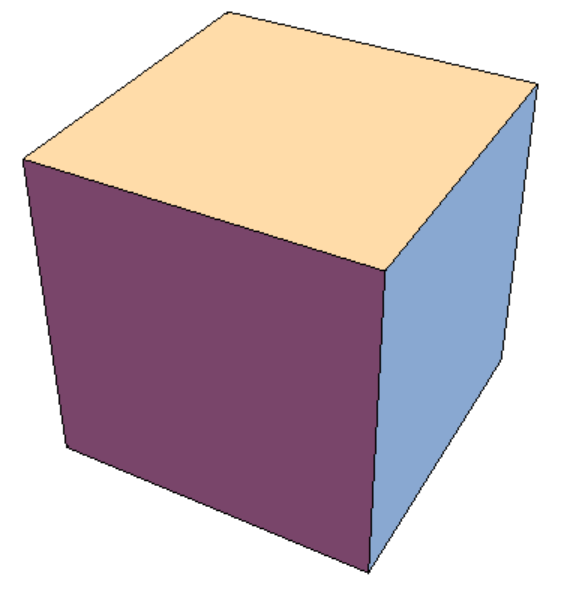
\includegraphics[width=0.3\textwidth]{figures/cube}
	\caption{A figure caption beneath the figure for description of the depicted concept which sometimes can be very long}
	\label{ft_fig_firstfig}
\end{figure}

In \autoref{ft_fig_firstfig}, for example, a PNG image is depicted (compiled with pdflatex). Alternatively, EPS figures can be embedded if dvips and ps2pdf compilation is used. All figures are listed in the list of figures with the command \imp{listoffigures}.

%%%%%%%%%%%%%%%%%%%%%%%%%%%%%%%%%%%%%%%%%%%%%%%%%%%%%%%%%%%
%%%%%%%%%%%%%%%%%%%%%%%%%%%%%%%%%%%%%%%%%%%%%%%%%%%%%%%%%%%

\section{Tables}

Data can be presented in tables, e.g., as shown in \autoref{ft_tab_ex}.

\begin{table}[!h]
	\centering
	\begin{tabular}{l|cl}
		\hline \hline
		
		& Property 1
		& Property 2\\ \hline
		Criterion 1
		& 764
		& 23546 \\
		Criterion 2
		& 3
		& 34 \\
		\hline \hline
	\end{tabular}
	\caption{Exemplary table}
	\label{ft_tab_ex}
\end{table}

Sometimes very long tables must be presented which may also go over pages. For this cases the packages \imp{longtable} is useful, as used in 

\begin{center}
	\begin{longtable}{l|l|l}
		
		% \baselinestretch{1.5}
		
		\hline \hline
		$i^3$ & $2i^3$ & $3i^3$ \bigstrut \\ \hline
		\endfirsthead
		
		\multicolumn{3}{c}{\tablename\ \thetable{} -- information message on top} \\
		\hline
		$i^3$ & $2i^3$ & $3i^3$ \bigstrut \\ \hline 
		\endhead
		
		\hline
		\multicolumn{3}{c}{Foot information} \\ \hline
		\endfoot
		
		\hline \hline
		\caption{Long Table}
		\label{lt}
		\endlastfoot
		
		1 & 2 & 3 \\
		8 & 16 & 24 \\
		27 & 54 & 81 \\
		64 & 128 & 192 \\
		125 & 250 & 375 \\
		216 & 432 & 648 \\
		343 & 686 & 1029 \\
		512 & 1024 & 1536 \\
		729 & 1458 & 2187 \\
		1000 & 2000 & 3000 \\
		1331 & 2662 & 3993 \\
		1728 & 3456 & 5184 \\
		2197 & 4394 & 6591 \\
		2744 & 5488 & 8232 \\
		3375 & 6750 & 10125 \\
		4096 & 8192 & 12288 \\
		4913 & 9826 & 14739 \\
		5832 & 11664 & 17496 \\
		6859 & 13718 & 20577 \\
		8000 & 16000 & 24000 \\
		9261 & 18522 & 27783 \\
		10648 & 21296 & 31944 \\
		12167 & 24334 & 36501 \\
		13824 & 27648 & 41472 \\
		15625 & 31250 & 46875 \\
		17576 & 35152 & 52728 \\
		19683 & 39366 & 59049 \\
		21952 & 43904 & 65856 \\
		24389 & 48778 & 73167 \\
		27000 & 54000 & 81000 \\
		29791 & 59582 & 89373 \\
		32768 & 65536 & 98304 \\
		35937 & 71874 & 107811 \\
		39304 & 78608 & 117912 \\
		42875 & 85750 & 128625 \\
		46656 & 93312 & 139968 \\
		50653 & 101306 & 151959 \\
		54872 & 109744 & 164616 \\
		59319 & 118638 & 177957 \\
		64000 & 128000 & 192000 \\
		68921 & 137842 & 206763 \\
		74088 & 148176 & 222264 \\
		79507 & 159014 & 238521 \\
		85184 & 170368 & 255552 \\
		91125 & 182250 & 273375 \\
		97336 & 194672 & 292008 \\
		103823 & 207646 & 311469 \\
		110592 & 221184 & 331776 \\
		117649 & 235298 & 352947 \\
		125000 & 250000 & 375000 \\
	\end{longtable}
\end{center}

All tables are listed with \imp{listoftables}.

%%%%%%%%%%%%%%%%%%%%%%%%%%%%%%%%%%%%%%%%%%%%%%%%%%%%%%%%%%%
%%%%%%%%%%%%%%%%%%%%%%%%%%%%%%%%%%%%%%%%%%%%%%%%%%%%%%%%%%%

\section{Enumerate and itemize}

If important sequential points are to presented the environment \imp{enumerate} can be used as follows:
\begin{enumerate}
	\item
	Some important stuff
	\item
	More stuff
\end{enumerate}
With the package \imp{enumerate} some options can be used, e.g.,
\begin{enumerate}[a)]
	\item
	Some important stuff
	\item
	More stuff
\end{enumerate}
or 
\begin{enumerate}[~~~1)]
	\item
	Some important stuff
	\item
	More stuff
\end{enumerate}

Alternatively, point can be just presented without any enumeration with the environment \imp{itemize}
\begin{itemize}
	\item
	Some important stuff
	\item
	More stuff
\end{itemize}

%%%%%%%%%%%%%%%%%%%%%%%%%%%%%%%%%%%%%%%%%%%%%%%%%%%%%%%%%%%
%%%%%%%%%%%%%%%%%%%%%%%%%%%%%%%%%%%%%%%%%%%%%%%%%%%%%%%%%%%
%%%%%%%%%%%%%%%%%%%%%%%%%%%%%%%%%%%%%%%%%%%%%%%%%%%%%%%%%%%

\chapter{Appendix, footnotes, todos and index}

%%%%%%%%%%%%%%%%%%%%%%%%%%%%%%%%%%%%%%%%%%%%%%%%%%%%%%%%%%%
%%%%%%%%%%%%%%%%%%%%%%%%%%%%%%%%%%%%%%%%%%%%%%%%%%%%%%%%%%%

\section{Appendix}

For many reasons some concept may be important for the document but too long for the main text. In this kind of cases these concept can be presented with the environment \imp{appendix} in appendices, e.g., as in \autoref{app_ex1} and \autoref{app_ex2}.

%%%%%%%%%%%%%%%%%%%%%%%%%%%%%%%%%%%%%%%%%%%%%%%%%%%%%%%%%%%
%%%%%%%%%%%%%%%%%%%%%%%%%%%%%%%%%%%%%%%%%%%%%%%%%%%%%%%%%%%

\section{Footnotes}

You may want to give additional information to some points\footnote{Bla bla} in the text\footnote{Blu blup}.

%%%%%%%%%%%%%%%%%%%%%%%%%%%%%%%%%%%%%%%%%%%%%%%%%%%%%%%%%%%
%%%%%%%%%%%%%%%%%%%%%%%%%%%%%%%%%%%%%%%%%%%%%%%%%%%%%%%%%%%

\section{Todos}

With the package \imp{todonotes} comments\todo{like this one}\ pointing to their place can be embedded into the text. These comments are veeeery useful if you are writing something for the first time or are working on a draft. The todos can be listed with \imp{listoftodos} where you want it to appear in order to see what is unfinished or needs some more work.

%%%%%%%%%%%%%%%%%%%%%%%%%%%%%%%%%%%%%%%%%%%%%%%%%%%%%%%%%%%
%%%%%%%%%%%%%%%%%%%%%%%%%%%%%%%%%%%%%%%%%%%%%%%%%%%%%%%%%%%

\section{Index}

If the document is very long, it may be very useful for a lot of readers to have an index for searching key words and certain concepts (Crtl+F is usually very helpful in PDFs but not always the best solution). For this, the  package \imp{makeidx}, the commands \imp{makeindex} and \imp{printindex} and the compiling option \imp{make index} are needed. You may want to index different words like heterogeneous materials\index{Heterogeneous materials}, effective properties\index{Effective properties} and homogenization\index{Homogenization}.

%%%%%%%%%%%%%%%%%%%%%%%%%%%%%%%%%%%%%%%%%%%%%%%%%%%%%%%%%%%
%%%%%%%%%%%%%%%%%%%%%%%%%%%%%%%%%%%%%%%%%%%%%%%%%%%%%%%%%%%
%%%%%%%%%%%%%%%%%%%%%%%%%%%%%%%%%%%%%%%%%%%%%%%%%%%%%%%%%%%

\begin{appendix}
	
	%%%%%%%%%%%%%%%%%%%%%%%%%%%%%%%%%%%%%%%%%%%%%%%%%%%%%%%%%%%
	%%%%%%%%%%%%%%%%%%%%%%%%%%%%%%%%%%%%%%%%%%%%%%%%%%%%%%%%%%%
	
	\chapter{Just an example appendix}
	\label{app_ex1}
	
	%%%%%%%%%%%%%%%%%%%%%%%%%%%%%%%%%%%%%%%%%%%%%%%%%%%%%%%%%%%
	
	\section{Bla blup}
	
	Sme stuff
	\begin{equation}
	f(x) = \int_{\Omega} g(x) dx \ .
	\end{equation}
	
	%%%%%%%%%%%%%%%%%%%%%%%%%%%%%%%%%%%%%%%%%%%%%%%%%%%%%%%%%%%\\
	%%%%%%%%%%%%%%%%%%%%%%%%%%%%%%%%%%%%%%%%%%%%%%%%%%%%%%%%%%%
	
	\chapter{Another example}
	\label{app_ex2}
	
	%%%%%%%%%%%%%%%%%%%%%%%%%%%%%%%%%%%%%%%%%%%%%%%%%%%%%%%%%%%
	
	\section{More stuff}
	
	Bla bla.
	
\end{appendix}

%%%%%%%%%%%%%%%%%%%%%%%%%%%%%%%%%%%%%%%%%%%%%%%%%%%%%%%%%%%
%%%%%%%%%%%%%%%%%%%%%%%%%%%%%%%%%%%%%%%%%%%%%%%%%%%%%%%%%%%
%%%%%%%%%%%%%%%%%%%%%%%%%%%%%%%%%%%%%%%%%%%%%%%%%%%%%%%%%%%

%\bibliographystyle{plain}
\bibliographystyle{abbrvnat}
\bibliography{literature/library}

\listoffigures
\listoftables

\printindex

%%%%%%%%%%%%%%%%%%%%%%%%%%%%%%%%%%%%%%%%%%%%%%%%%%%%%%%%%%%
%%%%%%%%%%%%%%%%%%%%%%%%%%%%%%%%%%%%%%%%%%%%%%%%%%%%%%%%%%%
%%%%%%%%%%%%%%%%%%%%%%%%%%%%%%%%%%%%%%%%%%%%%%%%%%%%%%%%%%%

\end{document}

%%%%%%%%%%%%%%%%%%%%%%%%%%%%%%%%%%%%%%%%%%%%%%%%%%%%%%%%%%%
